% ACA WA2 - Task 1 (1.1-1.4). IEEE double-column, 2 pages.
% Todos os números vêm de task1/analise_resultados_t1.txt (medidos) e
% task1/valores_teoricos.txt (datasheets). Compilar: pdflatex relatorio_task1.tex (2x)
\documentclass[conference,10pt]{IEEEtran}
\usepackage[utf8]{inputenc}
\usepackage[T1]{fontenc}
\usepackage{graphicx,booktabs,amsmath}
\usepackage[hidelinks]{hyperref}
\setlength{\tabcolsep}{2.5pt}

\begin{document}
\title{Characterising Deucalion for a Variable-Coefficient 3D Jacobi Solver}
\author{\IEEEauthorblockN{Rodrigo Rocha (PG65437) and André Santos (PG65399)}
\IEEEauthorblockA{MEI/MCA -- Advanced Computer Architectures, University of Minho, Braga, Portugal}}
\maketitle

\begin{abstract}
We characterise the three Deucalion partitions with datasheets and our own microbenchmarks, build
FP32 rooflines for the AMD EPYC 7742 and the Fujitsu A64FX with ceilings chosen for the
variable-coefficient Jacobi kernel, and define the test protocol for Task~2. Measuring changed
three conclusions: the real clock puts the AMD peak 22\% above nominal, the A64FX divides
393$\times$ slower than its peak, and wrong NUMA placement costs 7--10$\times$ of bandwidth.
\end{abstract}

\section{Introduction}
The \emph{varcoef} solver updates each point with a 7-point stencil whose face conductivities are
harmonic means, $\kappa_{pq}=2k_pk_q/(k_p+k_q)$. The reference performs about 45~FLOP per point,
7 of them divisions (in double). Its sweep reads \texttt{u} and an \texttt{int} material id and
writes \texttt{u\_new}: 12 useful bytes per point (16 moved, with write-allocate), an operational
intensity (OI) of 45/12~=~3.75~FLOP/B. With the residual and the copy back to \texttt{u}, a full
iteration moves 28 useful bytes for 48~FLOP (1.71~FLOP/B), and the inner loop strides by one plane.
All runs used whole nodes, pinned threads and GCC~15.2 (\texttt{-march=znver2}, \texttt{-mcpu=a64fx}).

\section{Hardware characterisation (1.1)}
Table~\ref{tab:hw} sets vendor values~\cite{amd56305,a64fx,a100} and system queries
(\texttt{lscpu}, \texttt{numactl}, \texttt{nvidia-smi}, \texttt{cudaGetDeviceProperties}) against
our measurements. \emph{Peak}: independent FMA chains in registers, 12 (AMD) or 24 (A64FX), enough to
hide the measured FMA latency (5 and 9 cycles); 8 per thread at full occupancy on the GPU.
\emph{Bandwidth}: STREAM~\cite{stream} (best of 19) and our Triad agree within 1.5\%; LLC: Triad
with 2~MiB (AMD) or 256~KiB (A64FX) per thread. \emph{Latency}: 1-thread pointer chasing over a
random (Sattolo) cycle, which defeats prefetching. Values are medians of 10 runs after a warm-up;
IQR below 1.1\% (SGEMM: 5\%).

\begin{table}[!t]\centering\scriptsize
\caption{Platforms, FP32 per node: nominal / measured}\label{tab:hw}
\setlength{\tabcolsep}{1.6pt}
\resizebox{\columnwidth}{!}{\begin{tabular}{@{}lccc@{}}\toprule
 & \textbf{x86} & \textbf{ARM} & \textbf{A100} \\ \midrule
Node & Bull H262-Z61 & Fujitsu PRIMEHPC FX700 & -- \\
Device & 2$\times$AMD EPYC 7742 & Fujitsu A64FX & NVIDIA A100-SXM4 \\
Cores; FP32/cycle & 128 (Zen 2); 32/core & 48 (4 CMG); 64/core & 108 SM; 128/SM \\
Clock (GHz) & 2.25 / 2.81 & 2.0 / 2.0 & 1.41 / 1.41 \\
Peak (GFLOP/s) & 9216 / 11\,269 & 6144 / 6049 & 19\,500 / 19\,188 \\
L1d; L2 & 32 KiB; 512 KiB/core & 64 KiB; 8 MiB/CMG & 192 KiB/SM; 40 MiB \\
L3; LLC BW & 16 MiB/CCX; 5036 GB/s & --; 2680 GB/s & --; -- \\
Memory & 256 GiB DDR4 & 32 GiB HBM2 & 40 GB HBM2 \\
BW (GB/s) & 409.6 / 299 (224) & 1024 / 813 (606) & 1555 / 1274 \\
Lat. L1/L2/L3 (ns) & 1.2 / 3.6 / 10.1 & 2.5 / $\sim$25 & 27.6 / 150--305 \\
Lat. memory & $\sim$105 ns & 144 ns & $\sim$410 ns \\
NUMA nodes & 8 (NPS4) & 4 & -- \\ \bottomrule
\end{tabular}}\\[1pt]
\raggedright\scriptsize Memory BW without (with) write-allocate, STREAM; A100: Triad (no write-allocate).
\end{table}

\emph{What measuring revealed.} (i)~Under an all-core AVX2 load the EPYC runs at 2.81~GHz
(\texttt{perf}), not its 2.25~GHz base: 122\% of the nominal peak. The A100 reaches 1410~MHz only
under sustained load (a short test at its 1095~MHz application clock gave the scaled peak within
3\%). The peak depends on the \emph{real} clock. (ii)~The A64FX
kernel exposes no cache data; the latency curve recovered the 64~KiB L1, the 8~MiB L2 per CMG and
two TLB knees (1 and 64~MiB: 16 and 1024 entries of 64~KiB pages). (iii)~One AMD thread sees only its CCX's 16~MiB L3. (iv)~The A100 L2 is two 20~MiB halves; the far one doubles
latency.

\emph{Validation and problems found.} SGEMM (OpenBLAS; Fujitsu SSL2) reached
49\% and 65\% of the measured peak. On the AMD,
the LLVM-built OpenBLAS loads its own OpenMP runtime (\texttt{libomp}) next to our \texttt{libgomp},
so binding was erratic (once 15.7~GFLOP/s); removing it gained only 5\% at
$n=8192$, and the larger $n=16384$ reached 5558~GFLOP/s. We redid the A64FX L2 Triad (IQR 9\%: 6~MiB per CMG sat at the edge of the 8~MiB L2) and the
\texttt{zfill} STREAM, which our script had silently skipped.

\section{Roofline model (1.2)}
Fig.~\ref{fig:roof} draws both rooflines in one graph (Appendix~A of~\cite{roofline}) with measured
peaks and the best measured bandwidth (M4, no write-allocate). The ridge points move from 22.5 and
6.0~FLOP/B (nominal) to 38 (AMD) and 7.4 (A64FX); 50 and 10 with write-allocate. On the AMD the real clock (+22\%) and DDR4 at 73\% of nominal both push it right. At
the sweep OI (3.75) a \emph{parallel} version with the reference arithmetic (E1) is memory bound at
about 0.84~TFLOP/s (AMD) and 2.3~TFLOP/s (A64FX): HBM gives the A64FX 2.7$\times$ the bandwidth with
only 54\% of the AMD peak. The serial, strided reference sits far lower (Sec.~IV).

\begin{figure}[!t]\centering
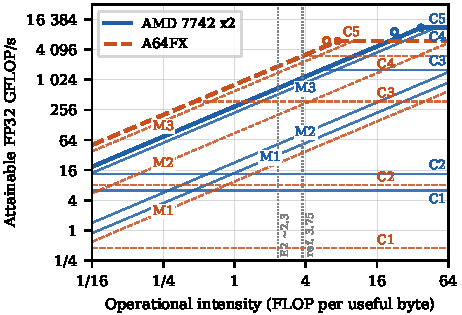
\includegraphics[width=0.88\columnwidth]{roofline.pdf}
\caption{Measured FP32 rooflines (thick) and ceilings of Table~\ref{tab:ceil} (thin). OI counts useful bytes. Filled/hollow dots: measured/nominal ridge points. Dotted: sweep OI
of the reference arithmetic (3.75) and of the pair-table version E2 ($\sim$2.3, 1-byte material).}\label{fig:roof}
\end{figure}

\section{Ceilings (1.3)}
As in~\cite{roofline}, ceilings go from what the reference gets (bottom) to what needs most effort
(top), the same on both machines (Table~\ref{tab:ceil}).

\begin{table}[!t]\centering\scriptsize
\caption{Ceilings, bottom to top (GFLOP/s, GB/s; measured)}\label{tab:ceil}
\begin{tabular}{@{}llrr@{}}\toprule
 & \textbf{Ceiling and why it applies to varcoef} & \textbf{AMD} & \textbf{A64FX} \\ \midrule
C1 & 7 divisions/point, scalar, 1 thread (reference) & 6.2 & 0.44 \\
C2 & scalar, 1 thread, no harmonic divisions (E2) & 13.5 & 8.0 \\
C3 & scalar, all cores (OpenMP) & 1589 & 379 \\
C4 & SIMD without FMA & 10\,536 & 3022 \\
C5 & SIMD + FMA (peak) & 11\,269 & 6049 \\ \midrule
M1 & stride of one plane (reference loop order) & 14 & 9.5 \\
M2 & wrong NUMA: all pages on node 0 (serial first touch) & 22.6 & 87.7 \\
M3 & with write-allocate (STREAM Triad) & 224 & 606 \\
M4 & without write-allocate & 299 & 813 \\ \bottomrule
\end{tabular}\\[1pt]
\raggedright\scriptsize C1 = scalar FP32 division rate $\times$ 45/7 (upper bound: the reference divides in
double). M1 = M3 $\times$ 4~B/line (64~B, 256~B). AMD M4 = $224\times32/24$; STREAM Copy (298) cannot
have write-allocate: it would move $298\times24/16=447>409.6$~GB/s.
\end{table}

\emph{Compute.} \textbf{C1} matters most for varcoef. Zen~2 issues one 8-lane \texttt{vdivps} every
3.5 cycles (measured, as in uops.info~\cite{uopsinfo}; \cite{amd56305} lists 5): 14$\times$ below the peak.
On the A64FX an SVE FP32 \texttt{FDIV} has a 98-cycle latency, is \emph{blocking} and runs only on
pipe FLA; the scalar one takes 29 cycles~\cite[Tables 16-2, 16-3]{a64fx}: 393$\times$ below the
peak. The serial reference reaches at most 9.9~Mpoints/s; even a 48-core SVE version keeping the 7
divisions (E1) is capped near 2.2~Gpoints/s, 23$\times$ below what HBM could feed. On the AMD,
vector divisions stay above the memory roof. The plain roofline hides this cost, hence C1
and strategy E2 (only 16 distinct $\kappa_{pq}$ for 4 materials, kept in L1). \textbf{C2/C3} remove divisions and add threads, but on the A64FX E2 stays division bound: its
final FDIV caps 48 cores near 15~Gpoints/s, 4$\times$ below HBM, so it needs a reciprocal estimate
(\texttt{FRECPE} + Newton).
\textbf{C4} differs by machine: Zen~2 has separate MUL/FMA and ADD pipes and keeps 93\% of the peak
without FMA, while each A64FX pipe does FMA \emph{or} MUL \emph{or} ADD and loses half.
\textbf{C5} is only partly attainable: the weighted sum maps to FMA, the rest does not.

\emph{Memory.} The OI counts useful bytes (no write-allocate, one element per access); M1 and M3
are effective-bandwidth ceilings for that count, so no traffic is counted twice. \textbf{M1}: with the reference loop order each load touches a new line and uses
1/16 (AMD) or 1/64 (A64FX) of it. One thread gets only 22 (AMD) or 50~GB/s (A64FX) from memory, so for the serial reference M1
drops to 1.4 and 0.8~GB/s. \textbf{M2}: STREAM under \texttt{numactl -{}-membind=0}, as when one
thread initialises the arrays, lost 9.8$\times$ (AMD) and 6.9$\times$ (A64FX), below what one node gives its own cores (remote
threads add fabric latency and contention): parallel first touch is mandatory. \textbf{M3/M4}: a normal store first reads the line (32~B moved, 24~B counted);
the A64FX \texttt{zfill} STREAM (\texttt{DC ZVA}) gains 34\%, exactly 32/24, and its Copy with
write-allocate moves $549.6\times24/16=824$~GB/s, the same as \texttt{zfill}. The order M1~$<$~M2~$<$~M3~$<$~M4 holds on both.

\section{Testing methodology for Task 2 (1.4)}
\emph{Protocol.} Exclusive nodes; modules loaded with explicit versions and logged with clock and
governor; threads pinned (\texttt{OMP\_PLACES=cores}); GCC~15.2, plus \texttt{fcc} on the A64FX and
\texttt{nvcc} (sm\_80) on the A100. One warm-up and 10 runs, reporting median and IQR (run times
have outlier tails that bias a mean). Cycles (\texttt{perf stat}) in every scaling run, as the AMD
clock drops from 3.38 to 2.81~GHz with core count. Time is measured without a profiler; each version
is checked against the reference output; a short \texttt{dev} run precedes every long job.
\emph{Profilers.} \texttt{perf} and PAPI exist on both CPUs, so their counters compare fairly;
vendor tools add what they miss: \texttt{fapp} on the A64FX (SVE use, energy) and Nsight
Systems/Compute on the A100 (transfers, occupancy). Energy: RAPL via \texttt{perf} (AMD),
\texttt{fapp} (A64FX), NVML (A100). \emph{Tests}: Table~\ref{tab:tests}.

\begin{table}[!t]\centering\scriptsize
\caption{Planned tests, metrics and expected outcome}\label{tab:tests}
\begin{tabular}{@{}lp{0.66\columnwidth}p{0.22\columnwidth}@{}}\toprule
T1 & Reference, 1 thread: time, MLUP/s, GFLOP/s, IPC & C1, M1 (1 thr.) \\
T2 & Strong scaling to 128/48 thr.\ (LLC-node, RAM): speedup & saturates at BW \\
T3 & Weak scaling (Gustafson): time at fixed points/thread & flat if BW scales \\
T4 & NUMA: serial/parallel first touch, close/spread & up to 7--10$\times$ (M2) \\
T5 & Vectorisation on/off, GCC vs.\ \texttt{fcc}: SIMD instr. & larger on A64FX \\
T6 & Misses, DRAM bytes $\Rightarrow$ measured vs.\ computed OI & loop order, reuse \\
T7 & Parallel overhead: barriers, residual reduction & cost of residual \\
T8 & Energy: J to solution, J/point, GFLOP/s/W & compare partitions \\
T9 & A100: kernel time, H2D/D2H, occupancy & BW vs.\ 1274 GB/s \\
T10 & Reference and best version on both rooflines & gap to ceilings \\ \bottomrule
\end{tabular}
\end{table}

\emph{Sizes} (12~B per point, $(n+2)^3$ grid) isolate one level of each machine: \textbf{L1}: $n=11$ on the AMD (25.7 of 32~KiB) and $n=14$ on the A64FX (48 of
64~KiB; $n=15$ is too tight for a 4-way cache). \textbf{LLC-1t} (1 thread): half of what one thread sees, above
the private levels: $n=86$ (7.8~MiB of a 16~MiB L3) and $n=68$ (3.9~MiB of an 8~MiB L2).
\textbf{LLC-node} (all threads; $n=86$ would leave 61~KiB per thread, an L2 test):
$n=250$ (183~MiB: 1.4~MiB per thread, 5.7~MiB per CCX) and $n=110$ (16~MiB: 343~KiB per thread,
4~MiB per CMG). \textbf{RAM}: $n=520$ on both (1.59~GiB; 1.19~GiB with a 1-byte material), not a power of two
(aliasing), within one CMG's 8~GiB.

{\let\footnotesize\scriptsize\begin{thebibliography}{6}
\bibitem{amd56305} AMD, ``Software Optimization Guide for AMD Family 17h Models 30h and Greater Processors,'' Pub.\ 56305, Advanced Micro Devices, 2020.
\bibitem{a64fx} Fujitsu, ``A64FX Microarchitecture Manual,'' v1.7, Fujitsu Ltd., May 2022.
\bibitem{a100} NVIDIA, ``NVIDIA A100 Tensor Core GPU Architecture,'' whitepaper, NVIDIA Corp., 2020.
\bibitem{stream} J.~D. McCalpin, ``Memory bandwidth and machine balance in current high performance computers,'' \emph{IEEE TCCA Newsletter}, pp.~19--25, Dec.\ 1995.
\bibitem{roofline} S.~Williams, A.~Waterman, and D.~Patterson, ``Roofline: an insightful visual performance model for floating-point programs and multicore architectures,'' Tech.\ Rep.\ UCB/EECS-2008-134, Univ.\ of California, Berkeley, Oct.\ 2008.
\bibitem{uopsinfo} A.~Abel and J.~Reineke, ``uops.info: characterizing latency, throughput, and port usage of instructions on Intel microarchitectures,'' in \emph{Proc.\ ASPLOS}, ACM, 2019, pp.~673--686; Zen~2 tables online at https://uops.info (accessed Nov.\ 2026).
\end{thebibliography}}
\end{document}
